% !TeX TS-program = pdflatex 

\documentclass[11pt,          % font size: 11pt or 12pt
               phd,           % degree:    ms or phd
               onehalfspacing % spacing: onehalfspacing or doublespacing
               ]{ncsuthesis}

%\documentclass[openany,oneside,titlepage,letterpaper]{book}

%%----------------------------------------------------------------------------%%
%%------------------------------ Import Packages -----------------------------%%
%%----------------------------------------------------------------------------%%
\usepackage{xcolor}
\usepackage{algorithm2e}
\usepackage{booktabs}  % professionally typeset tables
\usepackage{amsmath}
\usepackage{amsthm}
\usepackage{amssymb} 
\usepackage{amsfonts}
\usepackage{tikz}
\usepackage{tikz-qtree}
\usetikzlibrary{calc,positioning}
\usepackage{textcomp}  % better copyright sign, among other things
\usepackage{lscape}
\usepackage{longtable}
\usepackage{multirow}
\usepackage{subfig}    % composite figures
\usepackage{natbib}    % ability to use citet,citep
% \usepackage{fancyhdr}  % creates headers

\usepackage{siunitx} % For aligning numbers by decimal point

%%% For accessing system, OTF and TTF fonts
%%% (would have been loaded by polylossia anyway)
\usepackage{fontspec}
\usepackage{xunicode} %% loading this first to avoid clash with bidi/arabic

%%% For language switching -- like babel, but for xelatex
\usepackage{polyglossia}

\setmainlanguage{english}
\setotherlanguages{hindi,sanskrit} %% or other languages
\newfontfamily\devanagarifont[Script=Devanagari]{Noto Serif Devanagari}


%Citations should be of the form ``author year''  not ``author, year''
\bibpunct{(}{)}{;}{a}{}{,} % changes apalike bst into AMS format
 
%%----------------------------------------------------------------------------%%
%%---------------------------- Formatting Options ----------------------------%%
%%----------------------------------------------------------------------------%%
%%

%% -------------------------------------------------------------------------- %%
%% Disposition format -- any titles, headings, section titles
%%  These formatting commands affect all headings, titles, headings,
%%  so sizing commands should not be used here.
%%  Formatting options to consider are
%%     +  \sffamily - sans serif fonts.  Dispositions are often typeset in
%%                    sans serif, so this is a good option. 
%%     +  \rmfamily - serif fonts
%%     +  \bfseries - bold face
%\dispositionformat{\sffamily\bfseries}   % bold and sans serif
\dispositionformat{\bfseries}            % bold and serif

%% -------------------------------------------------------------------------- %%
%% Formatting for centered headings - Abstract, Dedication, etc. headings
%%  This is where one might put a sizing command.
%%  \MakeUppercase can be used to typeset all headings in uppercase.
\headingformat{\large\MakeUppercase}   % All letters uppercase
%\headingformat{\large}                % Not all uppercase
%\headingformat{\Large\scshape}        % Small Caps, used with serif fonts.

%% Typographers recommend using a normal inter-word space after
%% sentences. TeX's default is to add an wider space, but \frenchspacing
%% gives a normal spacing. Comment out the following line if you prefer wider spaces between sentences.
\frenchspacing

%% -------------------------------------------------------------------------- %%
%%  Optional packages
%%    A number of compatible packages to improve the look and feel of
%%    your document are available in the file optional.tex 
%%    (For example, hyperlinks, fancy chapter headings, and fonts)
%% To use these options, uncomment the next line and see optional.tex
%%  Optional Packages to consider.   These packages are compatible with
%%    ncsuthesis.  

%% -------------------------------------------------------------------------- %%
%% Fancy chapter headings
%%  available options: Sonny, Lenny, Glenn, Conny, Rejne, Bjarne
%\usepackage[Bjornstrup]{fncychap}
%\usepackage[Rejne]{fncychap}
%\usepackage[Sonny]{fncychap}
\newcommand{\headertitlefont}{%
    \fontsize{8}{12}\selectfont
}
\fancyhf{}
\fancyhead[L]{\headertitlefont \leftmark} %chapter
\fancyhead[R]{\headertitlefont \rightmark} %section
\fancyfoot[C]{\thepage} %footer
\pagestyle{fancy}     


%%----------------------------------------------------------------------------%%
%% Hyperref package creates PDF metadata and hyperlinks in Table of Contents
%%  and citations.  Based on feedback from the NCSU thesis editor, 
%%  the links are not visually distinct from normal text (i.e. no change
%%  in color or extra boxes).
\usepackage[xindy,acronym,toc]{glossaries}


%% -------------------------------------------------------------------------- %%
%% Microtype - If you use pdfTeX to compile your thesis, you can use
%%              the microtype package to access advanced typographic
%%              features.  By default, using the microtype package enables
%%              character protrusion (placing glyphs a hair past the right 
%%              margin to make a visually straighter edge)
%%              and font expansion (adjusting font width slightly to get 
%%              more favorable justification).
%%              Using microtype should decrease the number of lines
%%              ending in hyphens.
\usepackage{microtype}


%%----------------------------------------------------------------------------%%
%% Fonts 

%% ETD guidelines don't specify the font.  You can enable the fonts
%%  by uncommenting the appropriate lines.  Using the default Computer 
%%  Modern fonts is *not* required.  A few common choices are below.
%%  See http://www.tug.dk/FontCatalogue/ for more options.

%% Serif Fonts -------------------------------------------------
%%  The four serif fonts listed here (Utopia, Palatino, Kerkis,
%%  and Times) all have math support.


%% Utopia
%\usepackage[T1]{fontenc}
%\usepackage[adobe-utopia]{mathdesign}

%% Palatino
% \usepackage[T1]{fontenc}
% \usepackage[sc]{mathpazo}
% \linespread{1.05}

%% Kerkis
% \usepackage[T1]{fontenc}
% \usepackage{kmath,kerkis}

%% Times
% \usepackage[T1]{fontenc}
% \usepackage{mathptmx}


%% Sans serif fonts -------------------------

%\usepackage[scaled]{helvet}  % Helvetica
%\usepackage[scaled]{berasans} % Bera Sans

\setcounter{tocdepth}{3}
\setcounter{secnumdepth}{4}

%% https://www.overleaf.com/learn/latex/Theorems_and_proofs
% \newtheorem{theorem}{Theorem}[section]
% \newtheorem{corollary}{Corollary}[theorem]
% \newtheorem{lemma}[theorem]{Lemma}
\tikzset{
    grow'=down,
    level distance=42pt,
    % sibling distance=24pt,
    % sibling distance=8mm/#1,
    level/.style={sibling distance=3pt+44pt/(#1*#1*0.75)},
    edge from parent/.append style={
        draw,
        %thick,
        edge from parent path={
        (\tikzparentnode.west) |- ($(\tikzparentnode.west)!0.5!(\tikzchildnode.east)$) -| (\tikzchildnode.east)
        },
    },
    every node/.append style={
        anchor=center,
        rotate=90,
        draw=black,
        fill=white,
        thick,
        font=\footnotesize\bfseries,
        text centered,
        inner sep=0pt
    },
    var/.style={
        shape=circle,
        minimum height=16pt,
    },
    and/.style={
    and gate US,
    },
  not/.style={
    not gate US,
  },  
  or/.style={
    or gate US,
  },
  vot/.style={
    or gate US,
  }
}

%solve bug from fancyhdr in optional
%http://nw360.blogspot.com/2006/11/latex-headheight-is-too-small.html
%\setlength{\headheight}{26.94345pt} % corrected error in Overleaf
%\fancyhead[L]{\vspace{1mm}} % only puts chapter title in headers

%%----------------------------------------------------------------------------%%
%%---------------------------- Content Options -------------------------------%%
%%----------------------------------------------------------------------------%%
%% Size of committee: 3, 4, 5, or 6 -- this number includes the chair
\committeesize{4}

%% Members of committee
%%  Each of the following member commands takes an optional argument
%%   to specify their role on the committee.
%%  For co-chairs, use the commands:
%%      \cochairI{Doug Dodd}
%%      \cochairII{Chris Cox}
%%
\chair{Dr. Mihai A. Diaconeasa}
\memberII{Dr. Yousry Azmy}
\memberI{Dr. Aydin Aysu}
\memberIII{Dr. Nam Dinh}   % unnecessary if committeesize=3
% \memberIV{Member 4 name}    % unnecessary if committeesize=3, 4

%% Student writing thesis, \student{First Middle}{Last}
\student{Arjun}{Earthperson} % a full middle name

%% Degree program e.g. Marine, Earth, and Atmospheric Science
\program{Nuclear Engineering}

%%!!!!!! To Change Year !!!!!!%%
% If year of graduation is not same as current year (common for December graduates
% thanks to the Grad Schools odd graduation rules) go into ncsuthesis.cls and change 
% \the\year in the line:
% \newcommand{\ncsu@year}{\the\year}
% to the year of graduation. E.g.:
% \newcommand{\ncsu@year}{2020}

%% Thesis Title
%%  Keep in mind, according to ETD guidelines:
%%    +  Capitalize first letter of important words.
%%    +  Use inverted pyramid shape if title spans more than one line.
%%
%%  Note: To break the title onto multiple lines, use \break instead of \\.
% \thesistitle{A North Carolina State University Sample \LaTeX{} Thesis \break 
% with a Title So Long it Needs a Line Break}

% \thesistitle{A Sampling Scheme for Numerical Integration of Boolean Functions with Many Variables}

% \thesistitle{Finding Slopes in Large Boolean Spaces using Probabilistic Circuits}

% \thesistitle{Quantifying Risk by Simulating Probabilistic Circuits}

\thesistitle{A Data-Parallel Monte Carlo Framework for Large-Scale PRA using Probabilistic Circuits}
%% Degree year. Necessary if your degree year doesn't equal the current year.
\degreeyear{2025}

%% While your here make sure to change the PDF characteristics in optional.tex!!!

%%----------------------------------------------------------------------------%%
%%---------------------------- Personal Macros -------------------------------%%
%%----------------------------------------------------------------------------%%

%% A central location to add your favorite macros.

%% A few examples to get you started.
\newcommand{\uv}[1]{\ensuremath{\mathbf{\hat{#1}}}}
\newcommand{\bo}{\ensuremath{\mathbf{\Omega}}}
\newcommand{\eref}[1]{Eq.~\ref{#1}}
\newcommand{\fref}[1]{Fig.~\ref{#1}}
\newcommand{\tref}[1]{Table~\ref{#1}}

\theoremstyle{definition}
\newtheorem{definition}{Definition}[section]

%\makeglossaries

\newglossaryentry{cutset}
{
    name=Cut Set,
    description={A set of basic events (component failures) whose simultaneous occurrence causes the system to fail. In other words, the failure of all components in the set results in system failure.}
}

\newglossaryentry{pathset}
{
    name=Path Set,
    description={A set of components whose simultaneous functioning ensures system success. That is, if all components in the set are operational, the entire system functions properly.}
}

\newacronym{mcs}{MCS}{Minimal Cut Set}

\newglossaryentry{minimalcutset}
{
    name=Minimal Cut Set,
    description={A smallest possible Cut Set where the failure of all components causes system failure, and removing any component from the set would no longer result in system failure.},
    parent=cutset
}

\newacronym{mps}{MPS}{Minimal Path Set}

\newglossaryentry{minimalpathset}
{
    name=Minimal Path Set,
    description={A smallest possible Path Set where the functioning of all components ensures system success, and removing any component from the set would no longer ensure system success.},
    parent=pathset
}

\newglossaryentry{maximalpathset}
{
    name=Maximal Path Set,
    description={A Path Set that cannot be extended by adding more components; it includes all components that can be in a Path Set without redundancy. Adding any additional component does not create a new Path Set, as it would not change the system's operational status.}
}

\newacronym{pi}{PI}{Prime Implicant}

\newglossaryentry{primeimplicant}
{
    name=Prime Implicant,
    description={An implicant of a Boolean function that is as large as possible (in terms of combining variables) without containing redundant literals. It represents a minimal product term that cannot be combined further to simplify the function.},
    sort=Prime Implicant
}

\newacronym{epi}{EPI}{Essential Prime Implicant}

\newglossaryentry{essentialprimeimplicant}
{
    name=Essential Prime Implicant,
    description={A Prime Implicant that covers one or more minterms (true outputs) of a Boolean function that no other Prime Implicant covers. These are critical for the minimal expression of the function, as omitting them would alter the function's output.},
    parent=primeimplicant
}

\newacronym{et}{ET}{Event Tree}
\newglossaryentry{eventtree}{
    name=Event Tree,
    description={A logic diagram that begins with an initiating event or condition and progresses through a series of branches that represent expected system or operator performance that either succeeds or fails and arrives at either a successful or failed end state.},
}

\newacronym{PRA}{PRA}{Probabilistic Risk Assessment}
\newglossaryentry{pra}{
    name=Probabilistic Risk Assessment,
    description={A qualitative and quantitative assessment of the risk associated with plant operation and maintenance that is measured in terms of frequency of occurrence of risk metrics, such as release category frequency and its effects on the health of the public (also referred to as a PSA)},
}

% \newdualentry{et} % label
%   {ET}            % abbreviation
%   {Event Tree}  % long form
%   {A logic diagram that begins with an initiating event or condition and progresses through a series of branches that represent expected system or operator performance that either succeeds or fails and arrives at either a successful or failed end state} % description
  
% \glsaddall %  to list all entries <<<<<
% \usepackage[toc]{glossaries}
%\makeglossaries
%\glsaddall %  to list all entries <<<<<


%%---------------------------------------------------------------------------%%
\begin{document}
%%---------------------------------------------------------------------------%%
\frontmatter


%% ------------------------------ Dissertation Abstract ---------------------------------- %%
%% Dissertation Title: A Data-Parallel Monte-Carlo Framework for Large-Scale PRA using Probabilistic Circuits
\begin{abstract}
Probabilistic risk assessment (PRA) for nuclear systems typically requires enumerating minimal cut sets or essential prime implicants to capture all possible sequences of component failures, an approach that grows exponentially more complicated for large models. Existing methods combat this complexity by imposing structural restrictions on logic gates, applying rare-event approximations, or using bounding techniques like the min-cut upper bound. In this dissertation, we propose a data-parallel Monte Carlo framework that directly estimates probability distributions over entire Boolean spaces, circumventing many of the constraints faced by standard cut set analyses. By sampling from component-level input distributions rather than symbolically evaluating each logic configuration, our approach quantifies both success and failure events in one pass. Our open-source framework, Canopy, packs component states into integer bit-vectors and uses vectorized bitwise operations to achieve high throughput across modern GPUs, multi-core CPUs, and FPGAs. As an extension, we introduce a technique for sampling partial-derivatives using bitwise operations, which provides a pathway towards future work on gradient-based updates and other learning-based tasks.

We verify our implementation against the Aralia dataset, comparing convergence and accuracy with the open source SCRAM tool. Preliminary results demonstrate that with the exception of rare-events, data-parallel Monte Carlo, which is primarily memory-bound, can sample a few hundred million events in under 300ms while fully saturating available resources, even on older-generation consumer GPUs. For fault trees with a hundreds of events, sampling achieves error margins comparable to exact solvers. However, specialized variance-reduction or importance-sampling strategies remain essential for capturing extremely rare events with adequate precision.

We anticipate ongoing work on benchmarking the generic pressurized water reactor PRA model, in comparison with industry-standard tools (CAFTA, FTREX, SAPHIRE, XFTA), to provide further insights into solver performance and bottlenecks as the PRA model scales. 
\end{abstract}
\section*{An Informal Overview}
Probabilistic risk assessment (PRA) for nuclear systems requires evaluating complex Boolean functions that represent failure scenarios across thousands of components in two main steps: identifying minimal cut sets (the smallest sets of conditional events leading to end states of interest) and estimating the likelihood of these end states given component reliabilities. Although additional steps exist, PRA quantification primarily revolves around these tasks, which are computationally burdensome because exact solutions involve exhaustive inclusion-exclusion calculations that grow exponentially with the number of components, making large-scale analyses intractable. In response, many approximations have emerged: restricting model logic to a limited set of gate-types, describing only the failure space, applying probability truncation schemes like the rare-event approximation, or employing bounding methods such as the min-cut upper bound. Yet, even with these strategies, PRA quantification remains unwieldy in practice, demanding careful model management and tempered expectations regarding both accuracy and runtime.
% \vspace{-4mm}
\subsection*{Core Rationale - Building a Probability Estimator}
We propose a data-parallel Monte Carlo (MC) scheme that samples directly from input component-reliability distributions. Rather than generating every possible failure combination, we focus on random draws of the system’s global state, then tally how often particular sequences lead to an end state of interest. This sampling-based approach trades the intrinsic explosion of inclusion-exclusion terms with an exponential number of sample draws. This approach can accommodate a wider range of logic gates and event dependencies while putting the analyst in control of convergence. To unify these ideas, we use the concept of probabilistic circuits. Here, probability flow is represented as a structured computation graph over Boolean logic, but crucially, each gate’s input distributions come from random samplers rather than a symbolic enumeration of all possible states. This allows the circuit to model both failures and successes while keeping the model size manageable. However, MC approaches for PRA model quantification are not new. The key design principle rests on a massively parallel, hardware accelerated sampling scheme. By encoding component states in compact bit vectors, we exploit hardware-level parallelism. Boolean logic gates, including primitives and complex logic such as K/N translate into efficient bitwise operations. These operations are performed as a computation graph defined by the logic structure of the PRA model itself. We implemented the framework in an open-source tool named Canopy, which is built with SYCL to promote code portability across consumer GPUs, multi-core CPUs, or specialized accelerators like FPGAs.

\subsection*{The Role of Partial Derivatives}
One notable benefit of modeling probability distributions over the entire Boolean space is the ability to compute partial derivatives using the Shannon decomposition. Conceptually, the Shannon decomposition defines the derivative of Boolean function f(x), with respect to a subset of inputs. It is efficiently evaluated as a combination of bitwise XOR operations. Our approach samples from computation graphs representing arbitrary Boolean functions, including partial derivatives or more complex operations. This has immediate use for computing not only the conventional Birnbaum importance measure (which indicates how sensitive a system’s failure probability is to a component’s reliability) but also expanding to multi-component subsets. Additionally, since derivatives allow for gradient-based optimizations, there is potential for future work bridging advanced PRA and emerging machine-learning techniques. By embedding an auto-differentiation layer in the MC pipeline, one can imagine learning gate probabilities or even partial system structures from operational data, with the same data-parallel routines driving updates to reliability estimates.

\subsection*{Limitations}
\subsubsection*{Sampling Rare Events}
Ensuring accurate estimates for extremely low-probability events demands careful convergence criteria. In typical nuclear safety analyses, component failures can be vanishingly rare, so polling enough samples to capture these tail probabilities can prove challenging. Techniques such as importance sampling or other variance-reduction strategies may be needed to mitigate the slow convergence that arises when event likelihoods are measured in the range of 10\textsuperscript{-7} or lower. 

\subsubsection*{Sampling Correlated or Dependent Events}
A related concern is the treatment of common-cause failures (CCFs) and component dependencies. Characterizing CCF related failures or performing dependency analysis are important PRA activities. Future extensions of this framework thus require sampling from joint distributions, where correlated events are generated as a block. Integrating such dependent draws into bitpacked logic operations is feasible in principle but will require additional data-processing layers to ensure that correlated assignments remain both realistic and efficient to evaluate in large batches.

% \subsubsection*{Scaling Studies}
% Not all systems benefit from full-scale parallel sampling. For smaller PRA models (fewer components or simpler logic), existing approximate or event exact methods may remain faster and more transparent. A threshold likely exists at which the overhead of distributing computation across GPUs or multi-core CPUs outweighs the parallel advantages. Determining this floor for model size is an important empirical question.
 
% Probabilistic risk assessment (PRA) for nuclear systems relies on analyzing complex Boolean functions that capture failure scenarios spanning thousands of components. PRA quantification workflow involves identifying minimal cut sets and then estimating the probabilities of end states, yet exact methods are intractable for large models because they must evaluate an exponentially growing number of failure combinations. Approximations such as bounding techniques, truncations, logic simplification are often used to curb this computational blow-up, but they restrict model fidelity, omit success paths or subtle dependencies.

% We propose a generalized, data-parallel Monte Carlo (MC) framework that directly estimates probabilities over the entire Boolean space. By operating on input distributions $p(\mathbf{x})$ rather than enumerating minimal cut sets, our SYCL-based approach constructs probabilistic circuits to evaluate $P[f(\mathbf{x})]$ for arbitrary logic gates. This design:  
% 1) Trades exponential summations for an exponentially sampled state space, with the crucial freedom to stop sampling as soon as convergence criteria (user-defined tolerance) are met.  
% 2) Combines integer-bitpacked logic operations with data-parallel hardware acceleration (GPU, FPGA, or multi-core CPU), enabling millions of events to be sampled per second—even on modest consumer hardware.  
% 3) Avoids artificially high error from rare-event truncation by supporting importance sampling and variance reduction methods, improving estimates for extremely low-probability failure modes critical to nuclear safety.  
% 4) Fully decouples probability estimation from cut-set generation, making sense especially for massive PRA models where enumerating minimal cut sets is infeasible or unnecessary.  
% 5) Permits partial derivatives over Boolean functions, computed via Monte Carlo sampling of the Shannon decomposition (XOR events). This functionality underpins advanced sensitivity analyses (e.g., Birnbaum importance) for subsets of basic events—thereby bridging concepts from machine learning’s auto-differentiation into PRA.  

% We acknowledge that naive Monte Carlo can still converge slowly for extremely rare failures; hence, we outline variance reduction techniques and future work on sampling correlated events (e.g., common-cause failures) to address real-world dependencies. We also identify a practical lower bound on PRA model size where traditional methods may outperform our approach and discuss overhead trade-offs in deploying our open-source tool, Canopy, on single-GPU desktops versus distributed HPC clusters. Benchmarks against a generic pressurized water reactor PRA model confirm that, given suitably chosen convergence thresholds, data-parallel sampling can deliver orders-of-magnitude throughput gains relative to industry-standard tools (CAFTA, FTREX, SAPHIRE, SCRAM, XFTA) while maintaining accuracy within nuclear safety tolerances. Ultimately, this framework showcases a scalable path toward unifying tractable probabilistic models, hardware acceleration, and advanced reliability logic for next-generation PRA studies.

% \end{abstract}



% \chapter{A Brief and Informal Overview}
% \section*{Context}
% Probabilistic risk assessment (PRA) for nuclear systems requires the evaluation of complex Boolean functions representing failure scenarios across thousands of components. The evaluation is performed in two separate steps: (i) the identification of the smallest sets of conditional events leading to end states of interest (also called minimal cut sets), and (ii) an estimation of the likelihoods of these end states, given the state of knowledge of individual component reliabilities. Although there are additional steps, PRA quantification is an iterative process that revolves primarily around these tasks since they are computationally burdensome: exact solutions demand exhaustive inclusion-exclusion calculations that grow exponentially with the number of components. Therefore, the analysis of large-scale systems using exact methods remains intractable. 

% In response to these challenges, a generation of tools and methods has organically evolved around various approximations: they often restrict model definitions to a limited set of logic gates (commonly AND and OR), describe only the failure space by enumerating cut sets rather than prime implicants (thus omitting success paths), apply probability truncation schemes such as the rare-event approximation, or employ bounding techniques like the min-cut upper bound (MCUB). In practical terms, PRA quantification remains unwieldy, demanding careful model management and tempered expectations regarding both accuracy and runtime.

% \section*{The Data-Parallel Monte Carlo Approach}
% In response, we propose a generalized, data-parallel framework that directly estimates probability distributions using known Monte-Carlo (MC) techniques. By operating on input probability distributions $P(\mathbf{x})$ rather than symbolic evaluation of $f(\mathbf{x})$, our approach constructs probabilistic circuits that estimate $P[f(\mathbf{x})]$ for Boolean functions, enabling simultaneous quantification of all event sequences in a PRA. In effect, we are trading exponential growth in inclusion-exclusion terms during probability estimation for an exponential number of MC samples, all while making fewer assumptions on the structure of the underlying logic model. By shifting from enumerating minimal cut sets to sampling the entire solution space, our goal is to manage complexity more flexibly, harness modern hardware acceleration, and enable additional features such as partial derivative–based sensitivity analysis.

% Since we can stop sampling at any time based on arbitrary convergence criteria, we can set accuracy targets (and not be limited to using the rare-event truncation). The mean of the expected value still converges to the exact solution, which means, in the general case, the computed probabilities, although still approximations, have less error than when using the rare-event or MCUB approaches.

% The benefits of adopting a sampling approach are many-fold. Event sequence frequencies can be estimated without computing minimal cut sets. This is beneficial when models are so large that BDDs/exact methods cannot be used for probability estimation, and computing minimal cut sets is not required or also infeasible. Sampling also makes it possible to generate correlated samples, which creates a path for future work on CCF and dependency analysis. In addition, using a SYCL-based architecture allows us to make gains in throughput using the latest GPU/FPGA and multi-core CPU hardware. PRA models are integer-bitpacked and logic operations expressed as vectorized bitwise hardware operations, so minimal pre-processing or logic model manipulation is needed. For example, logical K/N gates do not need to be expanded to primitive types, and any combination of logical operations are supported. The actual performance of any logic gate is hardware dependent, which leaves room for future/parallel work on hardware optimizations. The data-parallelism enables the evaluation of billions of events within seconds on older/previous gen consumer hardware. With such abundance of compute, we can perform Boolean derivatives by sampling on the Shannon decomposition. This opens up the ability to define partial derivatives, which we use to perform sensitivity analysis such as calculating importance measures for subsets of basic events. Another emergent effect is that since we can define gradients, the opportunity for parallel/future work on learning model parameters and structures opens up. In sum, by adopting a MC sampling approach, (1) we are able to relax coherence constraints, (2) simultaneously model success and failure, (3) decouple probability estimation from cut set calculation, (4) compute derivatives/gradients by sampling on the Shannon decomposition (XOR), which allows us to (5) perform sensitivity analysis by defining importance measures such as Birnbaum as vectorial derivatives on $f$, (6) all while developing a data-parallel framework and (7) paving the way for finding common ground between the machine-learning (tractable probabilistic model) and PRA communities.

% We demonstrate the stability of our approximation method in our SYCL-based, MIT licensed implementation, Canopy. We benchmark against the generic pressurized water reactor PRA model, comparing its performance and accuracy against industry-standard tools (CAFTA, FTREX, SAPHIRE, SCRAM, and XFTA). 

% Probabilistic risk assessment (PRA) for nuclear systems requires the evaluation of complex Boolean functions representing failure scenarios across thousands of components. The evaluation is performed in two separate steps: (i) the identification of the smallest sets of conditional events leading to end states of interest (also called minimal cut sets), and (ii) an estimation of the likelihoods of these end states, given the state of knowledge of individual component reliabilities. Although there are additional steps, PRA quantification is an iterative process that revolves primarily around these tasks because (a) together, they provide insights that feed into risk reduction activities, and (b), they are the most computationally burdensome because computing exact solutions requires evaluating an exponentially growing number of failure combinations. This means that analysis of large-scale systems using exact methods remains intractable. Existing approaches rely on approximations that restrict model definitions to a subset of logic gates (typically AND, OR logic), operate exclusively in the failure space by describing cut sets rather than prime implicants (often excluding success paths entirely), employ probability truncation schemes like the rare-event approximation, or use bounding techniques such as the min-cut upper-bound (MCUB). In practical terms, PRA analysis remains an unwieldy enterprise, requiring careful model management and sobering expectations of accuracy and runtime.

% In response, we propose a generalized, data-parallel framework that directly estimates probability distributions using known Monte-Carlo (MC) techniques. By operating on input probability distributions $P(\mathbf{x})$ rather than symbolic evaluation of $f(\mathbf{x})$, our approach constructs probabilistic circuits that estimate $P[f(\mathbf{x})]$ for Boolean functions, enabling simultaneous quantification of all event sequences in a PRA. In effect, we are trading exponential growth in inclusion-exclusion terms during probability estimation for an exponential number of MC samples, all while making fewer assumptions on the structure of the underlying logic model. Since we can stop sampling at any time based on arbitrary convergence criteria, we can set accuracy targets (and not be limited to using the rare-event truncation). The mean of the expected value still converges to the exact solution, which means, in the general case, the computed probabilities, although still approximations, have less error than when using the rare-event or MCUB approaches.

% The benefits of adopting a sampling approach are many-fold. Event sequence frequencies can be estimated without computing minimal cut sets. This is beneficial when models are so large that BDDs/exact methods cannot be used for probability estimation, and computing minimal cut sets is not required or also infeasible. Sampling also makes it possible to generate correlated samples, which creates a path for future work on CCF and dependency analysis. In addition, using a SYCL-based architecture allows us to make gains in throughput using the latest GPU/FPGA and multi-core CPU hardware. PRA models are integer-bitpacked and logic operations expressed as vectorized bitwise hardware operations, so minimal pre-processing or logic model manipulation is needed. For example, logical K/N gates do not need to be expanded to primitive types, and any combination of logical operations are supported. The actual performance of any logic gate is hardware dependent, which leaves room for future/parallel work on hardware optimizations. The data-parallelism enables the evaluation of billions of events within seconds on older/previous gen consumer hardware. With such abundance of compute, we can perform Boolean derivatives by sampling on the Shannon decomposition. This opens up the ability to define partial derivatives, which we use to perform sensitivity analysis such as calculating importance measures for subsets of basic events. Another emergent effect is that since we can define gradients, the opportunity for parallel/future work on learning model parameters and structures opens up. In sum, by adopting a MC sampling approach, (1) we are able to relax coherence constraints, (2) simultaneously model success and failure, (3) decouple probability estimation from cut set calculation, (4) compute derivatives/gradients by sampling on the Shannon decomposition (XOR), which allows us to (5) perform sensitivity analysis by defining importance measures such as Birnbaum as vectorial derivatives on $f$, (6) all while developing a data-parallel framework and (7) paving the way for finding common ground between the machine-learning (tractable probabilistic model) and PRA communities.

% We demonstrate the stability of our approximation method in our SYCL-based, MIT licensed implementation, Canopy. We benchmark against the generic pressurized water reactor PRA model, comparing its performance and accuracy against industry-standard tools (CAFTA, FTREX, SAPHIRE, SCRAM, and XFTA). 


%% PRA modeling -> PRA quantification -> 
%% we show it is more than this - sensitivities, etc
%% we approach from a more general framework, relaxing many PRA specific concerns, broadening, 
%% implementing, generalizing, optimizing. And only then, refocusing to PRA related outcomes, and show %% that we have gained a little more insight (we come bearing fruit)... And these are the fruits we bear..

%  Current PRA solvers face computational barriers when analyzing large-scale systems, as they must evaluate an exponentially growing number of failure combinations. To overcome these challenges, existing approaches rely on various approximations: they operate exclusively in the failure space by describing cut sets rather than prime implicants, employ probability truncation schemes like the rare-event approximation, or use bounding techniques such as the min-cut-upper bound. We propose a probabilistic framework that side-steps these challenges by directly estimating probability distributions over Boolean spaces rather than evaluating individual failure combinations.

% Our approach constructs probabilistic circuits that estimate $P[f(\mathbf{x})]$ for Boolean functions, enabling simultaneous quantification of all event sequences and fault trees in a PRA. By operating on input probability distributions $P(\mathbf{x})$ rather than symbolic evaluation of $f(\mathbf{x})$, we avoid the combinatorial explosion inherent in exact calculations. The method employs Monte Carlo sampling in a data-parallel architecture, trading exponential growth in inclusion-exclusion terms for controlled convergence through sampling.

% We demonstrate the stability of our approximation method and extend it to handle composite Boolean operations, including partial derivatives and convolutions through modular circuit design. This enables efficient calculation of key PRA metrics: importance measures can be computed with respect to any subset of success or failure events, not just individual basic events, while essential prime implicants are identified through minimal non-zero gradients in $f$. Our implementation, named Canopy, shows significant performance improvements when tested against the generic pressurized water reactor PRA model. Benchmarks against industry-standard tools (CAFTA, FTREX, SAPHIRE, SCRAM, and XFTA) demonstrate orders-of-magnitude speedup in quantifying sequences with millions of basic events, while maintaining accuracy within established tolerance limits for nuclear safety applications.

% \footnote{Minimal cut sets that include success paths are called essential prime implicants}

% We propose a probabilistic scheme for evaluating Boolean functions with many variables. An immediate application of such an approach is that, since it inherently builds a probability estimator $P[f(\mathbf{x})]$ for Boolean circuits, one is able to quantify all event sequences and logic trees in a probabilistic risk assessment (PRA) simultaneously. Sequences and top events with millions of basic events can be quantified within seconds.

% By developing an estimator-based framework that operates over input probability distributions, we circumvent the need to evaluate $f(\mathbf{x})$ symbolically. Instead, we build circuits to evaluate $P[f(\mathbf{x})]$ for known input probability distributions $P(\mathbf{x})$. By using Monte Carlo sampling, we side-step the combinatorial explosion inherent in the exact probability calculation of $P[f(\mathbf{x})]$. This trades the exponential increase in inclusion-exclusion terms for an exponential increase in the number of Monte Carlo samples, allowing iterative convergence toward the exact solution using a process that is inherently data-parallel.

% After demonstrating that our method for approximating $f(\mathbf{x})$ is stable, we extend our approach to arbitrary combinatorial circuits. Composite Boolean operations, such as partial derivatives and convolutions can be evaluated by cascading modular circuitry. From here on, PRA tasks of high practical value, such as calculating importance measures and performing sensitivity analysis become quite straightforward. Importance measures are expressed as gradient operations with respect to subsets of basic events. The calculation of essential prime implicants, a central problem in PRA quantification, is transformed to determining the smallest subset of $\mathbf{x}$ that results in a non-zero gradient in $f$.

% We benchmark our solver, named Canopy, on the generic pressurized water reactor PRA model, comparing against industry-leading event-tree and fault-tree quantification tools CAFTA, FTREX, SAPHIRE, SCRAM, and XFTA. 


% // note, we are not solving for all X, we don't need to, it's not our problem
% // we care about F when P(x) is bounded, to a certain extent.
% // we want to reframe the problem of evaluating $F(x)\forall x$ as a problem about evaluating $ \hat{F} = P(F); \forall P(x)$
% // the search space is fundamentally large, there is no getting around that
% // but for some problems [list a few types], where $x \in [0, 1]$ some $x$, so we reduce the 
% We propose a data-parallel Monte Carlo scheme for evaluating Boolean functions with many variables, addressing a central practical challenge in risk and reliability analysis. This approach has many benefits, 

% We extend this notion to the general family of Boolean functions, and demonstrate how complex operations, such as partial derivatives and convolutions can be computed efficiently. 

% Instead of symbolically computing a Boolean function $F$, we evaluate $F$ overdo this by developing an estimator-based framework for performing operations on which can be extended for their $n\textsuperscript{th}$ partial derivatives of Boolean expressions, our method effectively circumvents the combinatorial explosion inherent in exact computation techniques. The data-parallel nature of the proposed approach demonstrates exceptional scalability on current-gen consumer hardware.

% An immediate benefit of this approach is that it addresses long-standing needs within Probabilistic Risk Assessment (PRA) model quantification, where existing methods struggle with large-scale models due to computational complexity or scalability limitations. Often, larger models are unquantifiable. Or, they are quantiti 

% By transforming PRA tasks—such as quantifying event sequence probabilities and performing sensitivity analyses—into operations over stochastically computed derivatives of Boolean functions, we enable lower-latency, high-throughput, and accurate model quantification as compared to existing approaches. 
 
% We show how the proposed method is generalizable to a wide array of combinatorial problems across various scientific computing disciplines, including digital circuit design, cryptography, and more. 




%% ---------------------------- Copyright page ------------------------------ %%
%% Comment the next line if you don't want the copyright page included.
\makecopyrightpage

%% -------------------------------- Title page ------------------------------ %%
\pagenumbering{roman}
\setcounter{page}{1}
\maketitlepage

%% -------------------------------- Dedication ------------------------------ %%
% \begin{dedication}
% %\centering dedication\ldots
% \end{dedication}

% %% -------------------------------- Biography ------------------------------- %%
% \begin{biography}
% %bio \ldots
% \end{biography}

% %% ----------------------------- Acknowledgements --------------------------- %%
% \begin{acknowledgements}
% ack \ldots
% \end{acknowledgements}

% \addtocontents{toc}{\protect\contentsline{chapter}{List of Tables}{\pageref{tagforlistoftables}}}

% \addtocontents{toc}{\protect\contentsline{chapter}{List of Figures}{\pageref{tagforlistoffigures}}}








\thesistableofcontents
\thesislistoftables
\thesislistoffigures
% \addcontentsline{toc}{chapter}{List of Algorithms}
% \listofalgorithms
% \thesisacronyms
% \thesisdefinitions

%%---------------------------------------------------------------------------%%
\mainmatter
% Chapters can remove or add
% %\input{parts/0_intro/informal_overview}

\chapter{Introduction}
% The entire risk assessment enterprise can be summarized as the act of integrating/bounding uncertainties within what we know to be true. Putting scaffolding around the unknowns. Using the few knowns to better structure the unknowns. To give form to the unknown.
\section{Background \& Motivation}
Probabilistic risk assessment (PRA) aims to quantitatively evaluate the likelihood and severity of adverse events in safety-critical industries. Driven by seminal works such as WASH-1400 and subsequent regulatory guidance, PRA now serves as a cornerstone of risk-informed decision-making in nuclear engineering. A canonical feature of PRA is its reliance on  Boolean logic structures (fault trees and event trees) that characterize sequences of component failures and human actions leading to top-level undesirable outcomes. While such structures ensure thoroughness, the computational complexity of enumerating all failure paths grows exponentially in the number of components. Even moderate-scale reactor models may involve tens of thousands of basic events, rendering naive calculation of end-state probabilities intractable.

Over decades, analysts have adopted a series of approximations and bounding schemes to handle this combinatorial explosion. Strategies include rare-event approximations (which assume minimal overlap between failure sets), min-cut upper bounds (which treat all minimal cut sets as mutually exclusive), and restrictions on gate types to keep expansions manageable. Tools such as CAFTA, FTREX, SAPHIRE, SCRAM, and XFTA implement these methods and remain widely used in industry. Nonetheless, these approximations can lead to conservative estimations.

In recent years, the continued growth of computing power has encouraged reassessment of how PRA calculations can be modernized. Specifically, massively parallel hardware (e.g., GPUs and multi-core CPUs) has prompted the exploration of data-parallel methods. Monte Carlo sampling is a natural fit for parallelization: since each sample is independent, thousands or millions of system-state draws can be processed simultaneously to build empirical estimates of key probabilities. Straightforward sampling from component failures (rather than enumerating complex Boolean expansions) offers flexibility in modeling dependencies and higher-order correlations. The overarching purpose of this dissertation is to develop a data-parallel Monte Carlo framework for large-scale nuclear PRA, grounded in a GPU-friendly integer bit-packing approach and extended to advanced sensitivity analyses using partial derivatives via Shannon decomposition.
\section{Scope}
This work reexamines how to efficiently compute the failure probability of a large Boolean system while capturing a wide array of gate structures, potential dependencies, and partial derivatives for sensitivity. We concentrate on the following core questions:

\begin{itemize}
   \item How can large-scale PRA models be quantified without explicit minimal cut set enumeration or strict reliance on model simplifications?
   \item Which data structures and numerical techniques allow us to exploit parallel hardware such as GPUs, multi-core CPUs, and field-programmable gate arrays (FPGAs)?
   \item What are the current limitations of Monte Carlo (e.g., rare-event estimation and common-cause failure sampling), and how might variance reduction or more sophisticated sampling schemes mitigate them?
\end{itemize}
While our emphasis centers on nuclear applications, the proposed techniques and software are equally suitable for other industries that manage complex risk scenarios (e.g., aerospace, chemical processing, or automotive safety). The dissertation does not attempt to unify every advanced PRA feature (e.g., dynamic simulations or large correlated uncertainties), but it lays the foundation for an extensible data-parallel approach that can incorporate such features in the future.

\clearpage
\section{Outline and Contributions}
The primary technical contributions of this dissertation can be summarized as follows:

\begin{enumerate}
\item \textbf{Data-Parallel Monte Carlo for Boolean Systems:}  
We introduce a new framework that estimates probabilities for all \emph{success} and \emph{failure} states in a single run of Monte Carlo sampling. By representing each random system state in a bit-packed data structure, we achieve high-throughput simulations where Boolean operators (AND, OR, \(k/n\), etc.) map naturally to bitwise operations on GPUs or multi-core CPUs.

\item \textbf{Integration with Probabilistic Circuits:}  
To unify event/fault tree logic with more flexible gate structures, we embed the model in a \emph{probabilistic circuit} representation. This perspective enables node-level factorization and sum mixtures, opening doors to advanced decomposition-based analyses while retaining parallel-friendly evaluation.

\item \textbf{Sampling Techniques for Partial-Derivatives:}  
We develop a bitwise algorithm to approximate partial derivatives of the system’s failure probability with respect to individual or clustered component reliabilities. By evaluating logical expressions under complementary assignments (as guided by the Shannon expansion), these derivatives can be computed in the same Monte Carlo pass. This capability facilitates advanced sensitivity and importance ranking in large models. It also opens a path towards integrating model evaluation with learning-based tasks.

\item \textbf{Benchmarking Against Industry Tools:}  
Through a series of case studies—most notably, the generic pressurized water reactor (PWR) reference model—we compare our approach with standard PRA tools (CAFTA, FTREX, SAPHIRE, SCRAM, XFTA). Results indicate that at comparable accuracy, our framework can surpass existing methods by orders of magnitude in runtime performance. We discuss how discrepancies in extremely low-probability events should be carefully monitored via convergence diagnostics.

\item \textbf{Prototype Implementation:}  
We present an open-source reference implementation named Canopy, built using the SYCL programming model. The code is portable across a variety of parallel architectures, including consumer GPUs and specialized accelerators. We provide usage examples and discuss future directions, such as unifying the approach with importance sampling to better handle rare events and building correlated sampling routines amenable to common-cause failure modeling.
\end{enumerate}

\section{Software Implementations}
\section{Related Publications}
\section{Organization of the Dissertation}
% The remainder of this dissertation is organized into multiple parts covering theoretical foundations, methodological frameworks, practical results, and future directions:

% \begin{itemize}
% \item \textbf{Part I: Foundations}  
%    – Provides an overview of rich Boolean representations (event trees, fault trees) in PRA, introduces probabilistic circuits, and reviews key Monte Carlo sampling principles relevant to reliability estimation.

% \item \textbf{Part II: Proposed Methods}  
%    – Details the data-parallel Monte Carlo approach, discussing bit-packed state encoding, gate-by-gate evaluation, and Shannon-decomposition-based partial derivatives.

% \item \textbf{Part III: Implementation and Results}  
%    – Documents the Canopy software design, GPU kernel formulations, and parallel performance optimizations. Presents numerical benchmarks against large PWR fault-tree models and comparisons with standard PRA codes. Highlights areas needing specialized variance reduction for rare events.

% \item \textbf{Part IV: Extensions and Conclusion}  
%    – Explores potential enhancements, such as correlated sampling for common-cause failures and ways to incorporate Bayesian or machine-learning-based parameter updates. Summarizes major findings and discusses the prospective impact of data-parallel quantification on future PRA methodologies.

% \end{itemize}

% \part{Foundations}

\chapter{Probabilistic Circuits}
\label{chap:boolean_prob_circuits}

\section{Boolean Functions}
\label{sec:boolean_functions}

Let \(\mathbf{x} = (x_1, x_2, \dots, x_n)\) be a vector of \(n\) Boolean variables, where each \(x_i \in \{0,1\}\). A \emph{Boolean function} is a map
\begin{equation}
\label{eq:boolean_function}
F(\mathbf{x}) \;=\; F(x_1, x_2, \dots, x_n) \;\in\; \{0,1\}.
\end{equation}
This function takes each possible configuration of \(\mathbf{x}\) (i.e., each element of \(\{0,1\}^n\)) to a single binary output in~\(\{0,1\}\). Boolean functions appear throughout digital logic, circuit design, and a wide range of computational applications.

For illustration, we can visualize small Boolean functions based on the size of \(\mathbf{x}\). For \(n=1\), there are two possible input states:

\begin{center}
\begin{tikzpicture}
\filldraw[black] (0,0) circle (2pt) node[anchor=north]{\small $x_1=0$};
\filldraw[black] (2,0) circle (2pt) node[anchor=north]{\small $x_1=1$};
\draw[->] (-0.5,0) -- (2.5,0);
\end{tikzpicture}
\end{center}

For \(n=2\), the four possible states can be positioned on a 2D lattice:

\begin{center}
\begin{tikzpicture}[scale=1.5]
\filldraw[black] (0,0) circle (2pt) node[anchor=north east]{\small $(0,0)$};
\filldraw[black] (1,0) circle (2pt) node[anchor=north west]{\small $(1,0)$};
\filldraw[black] (0,1) circle (2pt) node[anchor=south east]{\small $(0,1)$};
\filldraw[black] (1,1) circle (2pt) node[anchor=south west]{\small $(1,1)$};
\draw[->] (-0.5,0) -- (1.5,0);
\draw[->] (0,-0.5) -- (0,1.5);
\end{tikzpicture}
\end{center}

In three dimensions (\(n=3\)), the eight possible states correspond to the vertices of a cube:

\begin{center}
\begin{tikzpicture}[scale=2]
\coordinate (000) at (0,0,0);
\coordinate (001) at (0,0,1);
\coordinate (010) at (0,1,0);
\coordinate (011) at (0,1,1);
\coordinate (100) at (1,0,0);
\coordinate (101) at (1,0,1);
\coordinate (110) at (1,1,0);
\coordinate (111) at (1,1,1);

\foreach \point in {(000),(001),(010),(011),(100),(101),(110),(111)}
    \filldraw[black] \point circle (0.5pt);

\draw (000) -- (100) -- (110) -- (010) -- (000);
\draw (001) -- (101) -- (111) -- (011) -- (001);
\draw (000) -- (001);
\draw (100) -- (101);
\draw (110) -- (111);
\draw (010) -- (011);

\node[anchor=north east] at (000) {\small $(0,0,0)$};
\node[anchor=north west] at (100) {\small $(1,0,0)$};
\node[anchor=south east] at (010) {\small $(0,1,0)$};
\node[anchor=south west] at (110) {\small $(1,1,0)$};
\node[anchor=north east] at (001) {\small $(0,0,1)$};
\node[anchor=north west] at (101) {\small $(1,0,1)$};
\node[anchor=south east] at (011) {\small $(0,1,1)$};
\node[anchor=south west] at (111) {\small $(1,1,1)$};
\end{tikzpicture}
\end{center}

Boolean operators such as AND (\(\land\)), OR (\(\lor\)), and NOT (\(\lnot\)) allow constructing a wide variety of logical relationships. For example, in a setting where a system fails if any one of two components fails, the Boolean function can be written as
\[
F(x_A, x_B) \;=\; x_A \;\lor\; x_B.
\]
Here, \(F=1\) precisely when \(x_A=1\) or \(x_B=1\), encompassing a failure event if either component \(A\) or \(B\) is in state 1. More complex systems with many interdependent components may require Boolean functions with numerous variables and deeply nested operators.

Although Boolean functions are crucial for representing logical configurations, they operate purely in a binary framework and do not directly encode probability distributions. To include probabilistic behavior, we can move to a more expressive framework called \emph{probabilistic circuits}, which describe the distribution of variables in a directed acyclic graph (DAG). Such representations can capture both the combinatorial structure of system states and the uncertainty or likelihood associated with these states.

\section{Definition and Structure}

Consider a set of random variables \(\mathbf{X} = (X_1, X_2, \dots, X_n)\). A \emph{probabilistic circuit} \(\mathcal{C}\) is a DAG whose nodes consist of:

\begin{itemize}
 \item \textbf{Input nodes (leaves):} Each leaf encodes a base distribution over some subset of \(\mathbf{X}\). Often, these leaves correspond to univariate distributions \(p(X_i)\) or constant/indicator functions.
 \item \textbf{Internal nodes (gates):} Each gate combines incoming distributions from its children using either:
   \begin{itemize}
   \item \textbf{Sum-gates (mixture gates):} Weighted sums of child distributions, with nonnegative weights summing to 1.
   \item \textbf{Product-gates:} Factorized products of child distributions, each child covering disjoint subsets of \(\mathbf{X}\).
   \end{itemize}
\end{itemize}
The acyclic nature of the graph ensures that information flows consistently from the leaves toward a designated \emph{root} node.

\subsection{Sum-Gates and Product-Gates}

Let \(v\) be an internal node in \(\mathcal{C}\). Denote the children of \(v\) by \(\operatorname{ch}(v)\). Then:

\begin{itemize}
\item \textbf{Sum-gate:} Suppose \(v\) has children \(u_1,\dots,u_k\) with mixture weights \(\{\theta_{v,u_i}\}_{i=1}^k\) satisfying \(\sum_{i=1}^k \theta_{v,u_i} = 1\) and \(\theta_{v,u_i} \ge 0\). The distribution encoded at \(v\) is
\begin{equation}
\label{eq:sum_gate}
p_v(\mathbf{x}) \;=\; \sum_{i=1}^k \theta_{v,u_i}\,p_{u_i}(\mathbf{x}),
\end{equation}
where \(p_{u_i}(\mathbf{x})\) is the distribution encoded by child node \(u_i\).

\item \textbf{Product-gate:} Suppose \(v\) has children \(u_1,\dots,u_k\), each covering disjoint subsets of \(\mathbf{X}\). Let \(\mathbf{X}=\bigcup_{i=1}^k \mathbf{X}_{u_i}\) and \(\mathbf{X}_{u_i}\cap \mathbf{X}_{u_j} = \varnothing\) for \(i\neq j\). Then the distribution at \(v\) is
\begin{equation}
\label{eq:product_gate}
p_v(\mathbf{x})
\;=\;
\prod_{i=1}^k
p_{u_i}\bigl(\mathbf{x}_{u_i}\bigr),
\end{equation}
where \(\mathbf{x}_{u_i}\) is the restriction of \(\mathbf{x}\) to the variables in \(\mathbf{X}_{u_i}\).
\end{itemize}

\subsection{Leaf Nodes and the Circuit Distribution}

Each leaf node encodes a base distribution over its subset of variables (or a constant/indicator). Let \(v\) be a leaf node associated with \(p_v(\mathbf{X}_v)\). When the circuit is evaluated, each leaf contributes its assigned distribution or constant term. By recursively composing sum-gates and product-gates, every node \(v\) in the circuit defines a distribution \(p_v(\mathbf{x})\). The distribution of the entire circuit is given by evaluating its \emph{root} node \(r\):
\[
p_r(\mathbf{x}) \;=\; \text{(\(r\) evaluated from the leaves up)}.
\]

Probabilistic circuits unify structural and probabilistic modeling in a single formalism. They are widely used in fields such as artificial intelligence, machine learning, and automated reasoning, offering a tractable way to represent complex, high-dimensional probability distributions while preserving interpretable, compositional structure.


\input{parts/1_foundations/1_PRA/0_intro}
\input{parts/1_foundations/1_PRA/1_ET}
\input{parts/1_foundations/1_PRA/2_FT}


\usetikzlibrary {intersections}
\usetikzlibrary {graphs}
\begin{figure}[ht!]
\centering
\begin{tikzpicture}[domain=-4:12]
  % \draw [help lines] (-4,0) grid (12,12);
  \draw[->] (-4.0,0) -- (11,0) node[right] {$x$};
  \draw[->] (-4,0) -- (-4,12.0) node[above] {$f(x)$};
\begin{scope}[every node/.style={thick}]
    \node (ss_begin) at (-2.75,1.75) {$\text{S}_0$};

    \node (ss_end) at (9.5,11.0) {$\text{ES}_{0}$} ;
    % \node (ss_1) at (2.5,0.0) {$S_1$};
    % \node (ss_i) at (5.0,0.0) {$S_i$};
    % \node (ss_j) at (10.0,0.0) {$S_j$};
    % \node (ss_jp1) at (12.5,0.0) {$S_{j+1}$};

\end{scope}

\begin{scope}[>={Circle[black]},
              every edge/.style={draw=black,very thick}]
    % \path [->] (ss_0) edge (ss_1);
    % \path [->] (ss_1) edge (ss_i);
    % \path [->] (ss_i) edge (ss_j);
    % \path [->] (ss_j) edge (ss_jp1);
    % \path [->] (ss_jp1) edge (ss_f);
    % %\path [->] (B) edge node {$3$} (C);
    %\path [<->] (ss_begin) edge[out=25,in=220] node {} (ss_ie_i); 
    \path[<->,save path=\pathA,name path=A] (ss_begin) to [out=45,in=160, edge node={node [near end, above] {$\text{S}_0$}}](ss_end);

    \path[<->,save path=\pathB,name path=B] (1,0) to (1,11);

  \fill[name intersections={of=A and B}] (intersection-1) circle (3pt);

  \node[anchor=south east] (ss_ie_i) at (intersection-1) {$\text{IE}_i$};

  \draw[<->,black,very thick][use path=\pathA];
  %\draw[red] [use path=\pathB];
    %\path [<->] (ss_begin) edge[out=25,in=180] node[near end, above] {$\text{S}_0$} (ss_end); 
    %\path [<->] (ss_ie_i) edge[out=0,in=180] node[sloped] {} (ss_end); 
\end{scope}
\begin{scope}
  [grow'=right,
   level distance=50pt,
   every tree node/.append style={anchor=base west},
   execute at begin node=\strut,
   level 0/.style={sibling distance=0pt},  % initiating event
   level 1/.style={sibling distance=55pt}, %
   level 2/.style={sibling distance=45pt},
   level 3/.style={sibling distance=25pt, nodes={right=2}},
   edge from parent/.append style={
        draw,
        edge from parent path={
            (\tikzparentnode.east) -| ($(\tikzparentnode.east)!0.5!(\tikzchildnode.west)$) |- (\tikzchildnode.west)
        },
    },
    every node/.append style={anchor=center,font=\small,text centered},
    % every level 0 node/.append style={circle, font=\small\bfseries, draw, fill=blue!30, inner sep=0pt},
    every leaf node/.append style={nodes={right=2}},
   ]
   \graph
{
  "$I$"[at={(intersection-1)}, right=1.25] -> {
    b -> c
  };
};

  % \node at (intersection-1)[right=1.25]{$I$}
  %    child {node {$F_{1}^s$}
  %      child {node {$F_{2}^s$}
  %        child {node {$\text{ES}_{1}$}}
  %      }
  %      child {node {$F_{2}^f$}
  %        child {node {$\text{ES}_{2}$}}
  %        child {node {$\text{ES}_{3}$}}
  %      }
  %    }
  %    child {node  {$F_{1}^f$}
  %      child {node {$\text{ES}_{4}$}}

  \end{scope}   
\end{tikzpicture}
\end{figure}

\chapter{Probability Estimation using Monte Carlo Sampling}
\section{Monte Carlo Fundamentals}
Monte Carlo methods provide a versatile framework for approximating expectations, probabilities, and other quantities of interest by simulating random observations from an underlying distribution. At its core, a Monte Carlo estimator uses repeated random draws to approximate quantities such as
\begin{equation}
\label{eq:generic_monte_carlo_estimator}
\mathbb{E}[f(X)]
\;=\;
\int f(x)\,p(x)\,\mathrm{d}x
\;\;\approx\;\;
\frac{1}{N}\sum_{i=1}^N f\bigl(x^{(i)}\bigr),
\end{equation}
where \(x^{(1)},x^{(2)},\dots,x^{(N)}\) are independent and identically distributed (i.i.d.) samples drawn from \(p\). The function \(f\) is a measurable function of the random variable \(X\). In reliability and PRA contexts, \(f\) might be an indicator of a particular event (e.g., a system failure), in which case \(\mathbb{E}[f(X)]\) becomes the probability of that event.
\subsection{Convergence and the Law of Large Numbers}
A central theoretical result underpinning Monte Carlo sampling is the \emph{Law of Large Numbers (LLN)}. In one of its classical forms, the Strong LLN states:
\begin{theorem}[Strong Law of Large Numbers]
\label{thm:SLLN}
Let \(X_1, X_2, \dots\) be a sequence of i.i.d.\ random variables with finite expectation \(\mathbb{E}[X_1]\). Then, with probability 1,
\[
\lim_{N\to\infty}
\frac{1}{N}\sum_{i=1}^N X_i
\;=\;
\mathbb{E}[X_1].
\]
\end{theorem}
Applied to the sample estimator in Eq.~\eqref{eq:generic_monte_carlo_estimator}, the LLN implies that as the number of samples \(N\) grows large, the average of the function values \(f\bigl(x^{(i)}\bigr)\) converges to \(\mathbb{E}[f(X)]\). Thus, by simply drawing enough samples, one can approximate probabilities or expectations arbitrarily well (with probability~1).

\subsection{Central Limit Theorem and Error Analysis}
Another classical result is the \emph{Central Limit Theorem (CLT)}, which indicates that the Monte Carlo estimator’s distribution (around its true mean) approaches a normal distribution for large \(N\). Specifically,

\begin{theorem}[Central Limit Theorem]
\label{thm:CLT}
Suppose \(X_1, X_2,\dots\) are i.i.d.\ random variables with mean \(\mu=\mathbb{E}[X_1]\) and variance \(\sigma^2=\mathbb{V}[X_1]<\infty\). Then the sample mean satisfies
\[
\sqrt{N}
\biggl(
 \frac{1}{N}\sum_{i=1}^N X_i - \mu
\biggr)
\;\;\xrightarrow{\mathrm{d}}\;\;
\mathcal{N}(0,\sigma^2),
\]
where \(\xrightarrow{\mathrm{d}}\) denotes convergence in distribution.
\end{theorem}

In practical terms, the CLT implies that for sufficiently large \(N\), the sampling fluctuations of the Monte Carlo estimator around the true mean are approximately normal. The variance of this normal distribution decreases with \(1/N\). Therefore, one can estimate confidence intervals, standard errors, and convergence rates by tracking empirical variance across the sample.

The above principles remain valid even when \(f\) is an indicator of a Boolean event or a composite system failure embedded in an event/fault tree. One need only be able to draw samples \(\bigl(x^{(i)}\bigr)\) from the system’s joint distribution over basic events (or from any suitable representation of the PRA model) and then evaluate the function \(f\) to determine system success/failure for each sample. Subsequent chapters will expand on how these samples can be generated for event trees, fault trees, or more complex DAG-based representations.

\section{Random Number Generation and Random Variates}
Monte Carlo estimators rely on the ability to generate random realizations from a given distribution. Computers, however, do not typically provide true randomness; instead, they use \emph{pseudo}-random number generators (PRNGs) to produce sequences of numbers that mimic realizations from a uniform distribution on \([0,1]\). From these \emph{uniform} samples, one can then derive samples from more general distributions using various transformations (e.g., the \emph{inverse transform} method, acceptance-rejection, composition methods, or specialized sampling algorithms).

\subsection{Pseudo-Random Number Generation}
A PRNG is formally a deterministic function that, given an initial \emph{seed}, generates a long sequence of values in \((0,1)\). Popular choices include:
\begin{itemize}
\item \emph{Linear Congruential Generators (LCG)}, which use a recurrence of the form
\[
X_{n+1}
\;=\;
(a\,X_n + c)
\;\bmod\; m,
\]
then normalize \(\frac{X_{n+1}}{m}\) to produce a pseudo-random variate in \((0,1)\).
\item \emph{Mersenne Twister}, which generates high-quality pseudo-random numbers with a very long period (e.g., \(2^{19937}-1\)).
\item \emph{Philox} or other counter-based methods that deliver high performance and reproducible streams across parallel computations.
\end{itemize}

While these methods provide deterministic sequences, strong design ensures that the resulting outputs pass numerous statistical tests for randomness. If the seed is chosen randomly (or from a secure source), these methods can approximate uniformity closely enough for most Monte Carlo studies.

\subsection*{Random Variates via Transformations}
Given access to uniform samples \(U\sim \mathrm{Unif}(0,1)\), one can construct samples from many other distributions. Two widely used techniques are:

\begin{enumerate}
\item \textbf{Inverse Transform Sampling:}  
   Suppose a continuous variable \(X\) has cumulative distribution function (CDF) \(F_X(x)\). If \(U\sim \mathrm{Unif}(0,1)\), then \(X=F_X^{-1}(U)\) follows the same distribution as \(X\). More precisely,
   \[
   P\bigl[X \le x\bigr]
   \;=\;
   P\bigl[F_X^{-1}(U)\le x\bigr]
   \;=\;
   P\bigl[U \le F_X(x)\bigr]
   \;=\;
   F_X(x),
   \]
   provided \(F_X\) is continuous and strictly increasing.  

\item \textbf{Acceptance-Rejection:}  
   For certain distributions where the inverse CDF is not straightforward, one can sample from an easier \emph{proposal distribution} \(q(x)\) that bounds the targeted density \(p(x)\). Specifically, if \(p(x)\le M\,q(x)\) for all \(x\), then:
   \begin{enumerate}
   \item Draw \(Y\sim q(\cdot)\) and \(Z\sim \mathrm{Unif}(0,1)\).
   \item Accept \(Y\) if \(Z\le \frac{p(Y)}{M\,q(Y)}\). Otherwise, reject and repeat.
   \end{enumerate}
   The accepted sample \(Y\) follows distribution \(p(x)\).  
\end{enumerate}

\subsection{Boolean Events as Discrete Random Variables}
In PRA contexts, many variables are \emph{discrete}, often Bernoulli (success/failure) or categorical (e.g.\ multiple failure modes). Generating \(\{0,1\}\)-valued samples is then straightforward, since for each basic event \(b\),
\[
\Pr[b=1] \;=\; p(b),
\quad
\Pr[b=0] \;=\; 1-p(b).
\]
Given a uniform variate \(U\), one sets
\[
b
\;=\;
\begin{cases}
1, & U \le p(b),\\
0, & \text{otherwise}.
\end{cases}
\]
This approach naturally extends to multi-categorical events. More complex dependencies among events can also be captured by specifying appropriate conditional distributions.

\subsection{Extending Boolean Events to Continuous Random Variables}
A \emph{continuous} random variable \(Y\) has a probability density function (PDF) \(f_Y(y)\) on a continuous domain \(\mathcal{Y}\subseteq \mathbb{R}\). Common examples in reliability include:
\begin{itemize}
\item \textbf{Exponential Distribution}, often used to model times to failure under a constant hazard rate \(\lambda\). Its PDF is
\[
f_Y(y) \;=\; \lambda\, e^{-\lambda y},
\quad
y \ge 0.
\]
\item \textbf{Weibull Distribution}, with flexible shape parameter \(\beta>0\) and scale parameter \(\alpha>0\). Its PDF is
\[
f_Y(y)
\;=\;
\frac{\beta}{\alpha}
\Bigl(\frac{y}{\alpha}\Bigr)^{\!\beta -1}
\exp\!\biggl[-\bigl(y/\alpha\bigr)^{\!\beta}\biggr],
\quad
y\ge 0.
\]
\item \textbf{Lognormal Distribution}, where \(\log(Y)\) follows a normal distribution. This is sometimes employed for components whose lifetimes span multiple orders of magnitude.
\end{itemize}
In a PRA context, continuous random variables typically arise when modeling the \emph{time dimension}: for instance, the time until a valve sticks closed, or the moment when a pipe experiences a critical crack. One can then generate a Bernoulli indicator for whether the failure has occurred by time \(t\) using
\[
\Pr[Y \le t]
\;=\;
\int_{0}^{t} f_Y(y)\,\mathrm{d}y
\;=\;
F_Y(t),
\]
where \(F_Y\) is the cumulative distribution function (CDF) of \(Y\). Evaluating this probability at each Monte Carlo trial and comparing against a uniform random variate yields a discrete failure indicator. Hence, continuous distributions can be mapped to discrete states at any chosen time horizon.




\subsubsection*{Ensuring Reliable Sampling in High-Dimensional Boolean Spaces}
When dealing with large-scale PRA models or deeply nested Boolean structures (multiple fault trees and event trees), a careful approach to random variate generation is needed:
\begin{itemize}
\item \textbf{Reusable Streams:} Use a consistent seeding and PRNG strategy to ensure reproducibility of results, especially when comparing multiple system configurations.
\item \textbf{Parallel and Distributed Simulations:} Avoid overlapping random streams (i.e., ensure different parallel processes use uncorrelated seeds).
\item \textbf{Validation of Randomness:} Use standard test suites (e.g.\ TestU01, Diehard) if the model’s accuracy depends on fine-scale statistical properties.
\end{itemize}
Once random variates for each basic event are generated, higher-level logical structures (e.g.\ gates in a fault tree or branches in an event tree) can be evaluated deterministically.  Subsequent sections will address how to form either a single \emph{global} sample of all events in the system or to \emph{factorize} the sampling process according to the structure of the DAG-based PRA model.

\chapter{Problem Statement}


% \begin{figure}
% \begin{tikzpicture}
%   \graph [nodes={align=center, inner sep=1pt}, grow right=1.5]
% {
%   a,
%   b,
%   c -> d -> {
%     e -> f -> g,
%     h -> i
%   } -> j,
%   k -> l
% }
% \end{tikzpicture}
% \caption{An illustrative “success tree,” showing how multiple mitigation paths from the initial condition \(S_0\) can lead to safe or acceptable outcomes.}
% \label{fig:success_tree_example}
% \end{figure}
% Match the style from fig:event_tree_example
% \tikzset{grow'=right,level distance=48pt}
% %\tikzset{execute at begin node=\strut}
% %\tikzset{every tree node/.style={anchor=base west}}
% \tikzset{
%     edge from parent/.append style={very thick},
%     edge from parent/.style={
%         draw,
%         edge from parent path={
%             (\tikzparentnode.east) -| ($(\tikzparentnode.east)!0.5!(\tikzchildnode.west)$) |- (\tikzchildnode.west)
%         },
%     },
%     every node/.style={circle, minimum width=0.2cm, draw, anchor=center,font=\small\bfseries, text centered},
%     %every level 0 node/.style={circle, font=\small\bfseries, draw, fill=blue!30, inner sep=0pt},
%     %every internal node/.style={font=\small, inner sep=4pt},
%     %every leaf node/.style={rectangle, draw, fill=blue!30, minimum width=2.5cm, text centered},
%     %frontier/.style={distance from root=400pt},
% }
% \Tree [.\(1\)
%     [.\(F_1^{\text{fail}}\)
%         [.\(X_3\) ]
%     ]
% ]
% \Tree [.\(I\)
%     [.\(F_1^{\text{succ}}\)
%         [.\(F_2^{\text{succ}}\)
%             [.\(X_1\) ]
%         ]
%         [.\(F_2^{\text{fail}}\)
%             [.\(X_2\) ]
%         ]
%     ]
%     [.\(F_1^{\text{fail}}\)
%         [.\(X_3\) ]
%     ]
% ]
% Example success tree
% \Tree [.\(S_0\)
%     [.\(Mitigation \#1\)
%         [.\(Mitigation \#2\)
%             [.\(\text{Full Success}\) ]
%         ]
%         [.\(Alternate\)
%             [.\(\text{Partial Success}\) ]
%         ]
%     ]
%     [.\(Backup\)
%         [.\(\text{Alternate Success}\) ]
%     ]
% ]

% \part{A Brute Force Approach}
\large{\begin{hindi}
नर हो, न निराश करो मन को \\
कुछ काम करो, कुछ काम करो
\end{hindi}}
\chapter{Model Representation}

\input{parts/2_bruteforce/1_representation/1_DAG}
\input{parts/2_bruteforce/1_representation/2_alt_forms}
\chapter{Building a Data-Parallel Monte-Carlo Probability Estimator}

\input{parts/2_bruteforce/2_estimator/1_overview}

\input{parts/2_bruteforce/2_estimator/2_prng}

\section{Preliminary Benchmarks}

\input{parts/2_bruteforce/3_benchmark/3_table_aralia_ft_dataset}

\input{parts/2_bruteforce/3_benchmark/3_setup}

\clearpage
\begin{landscape}
\begin{figure}[h]
    \centering
    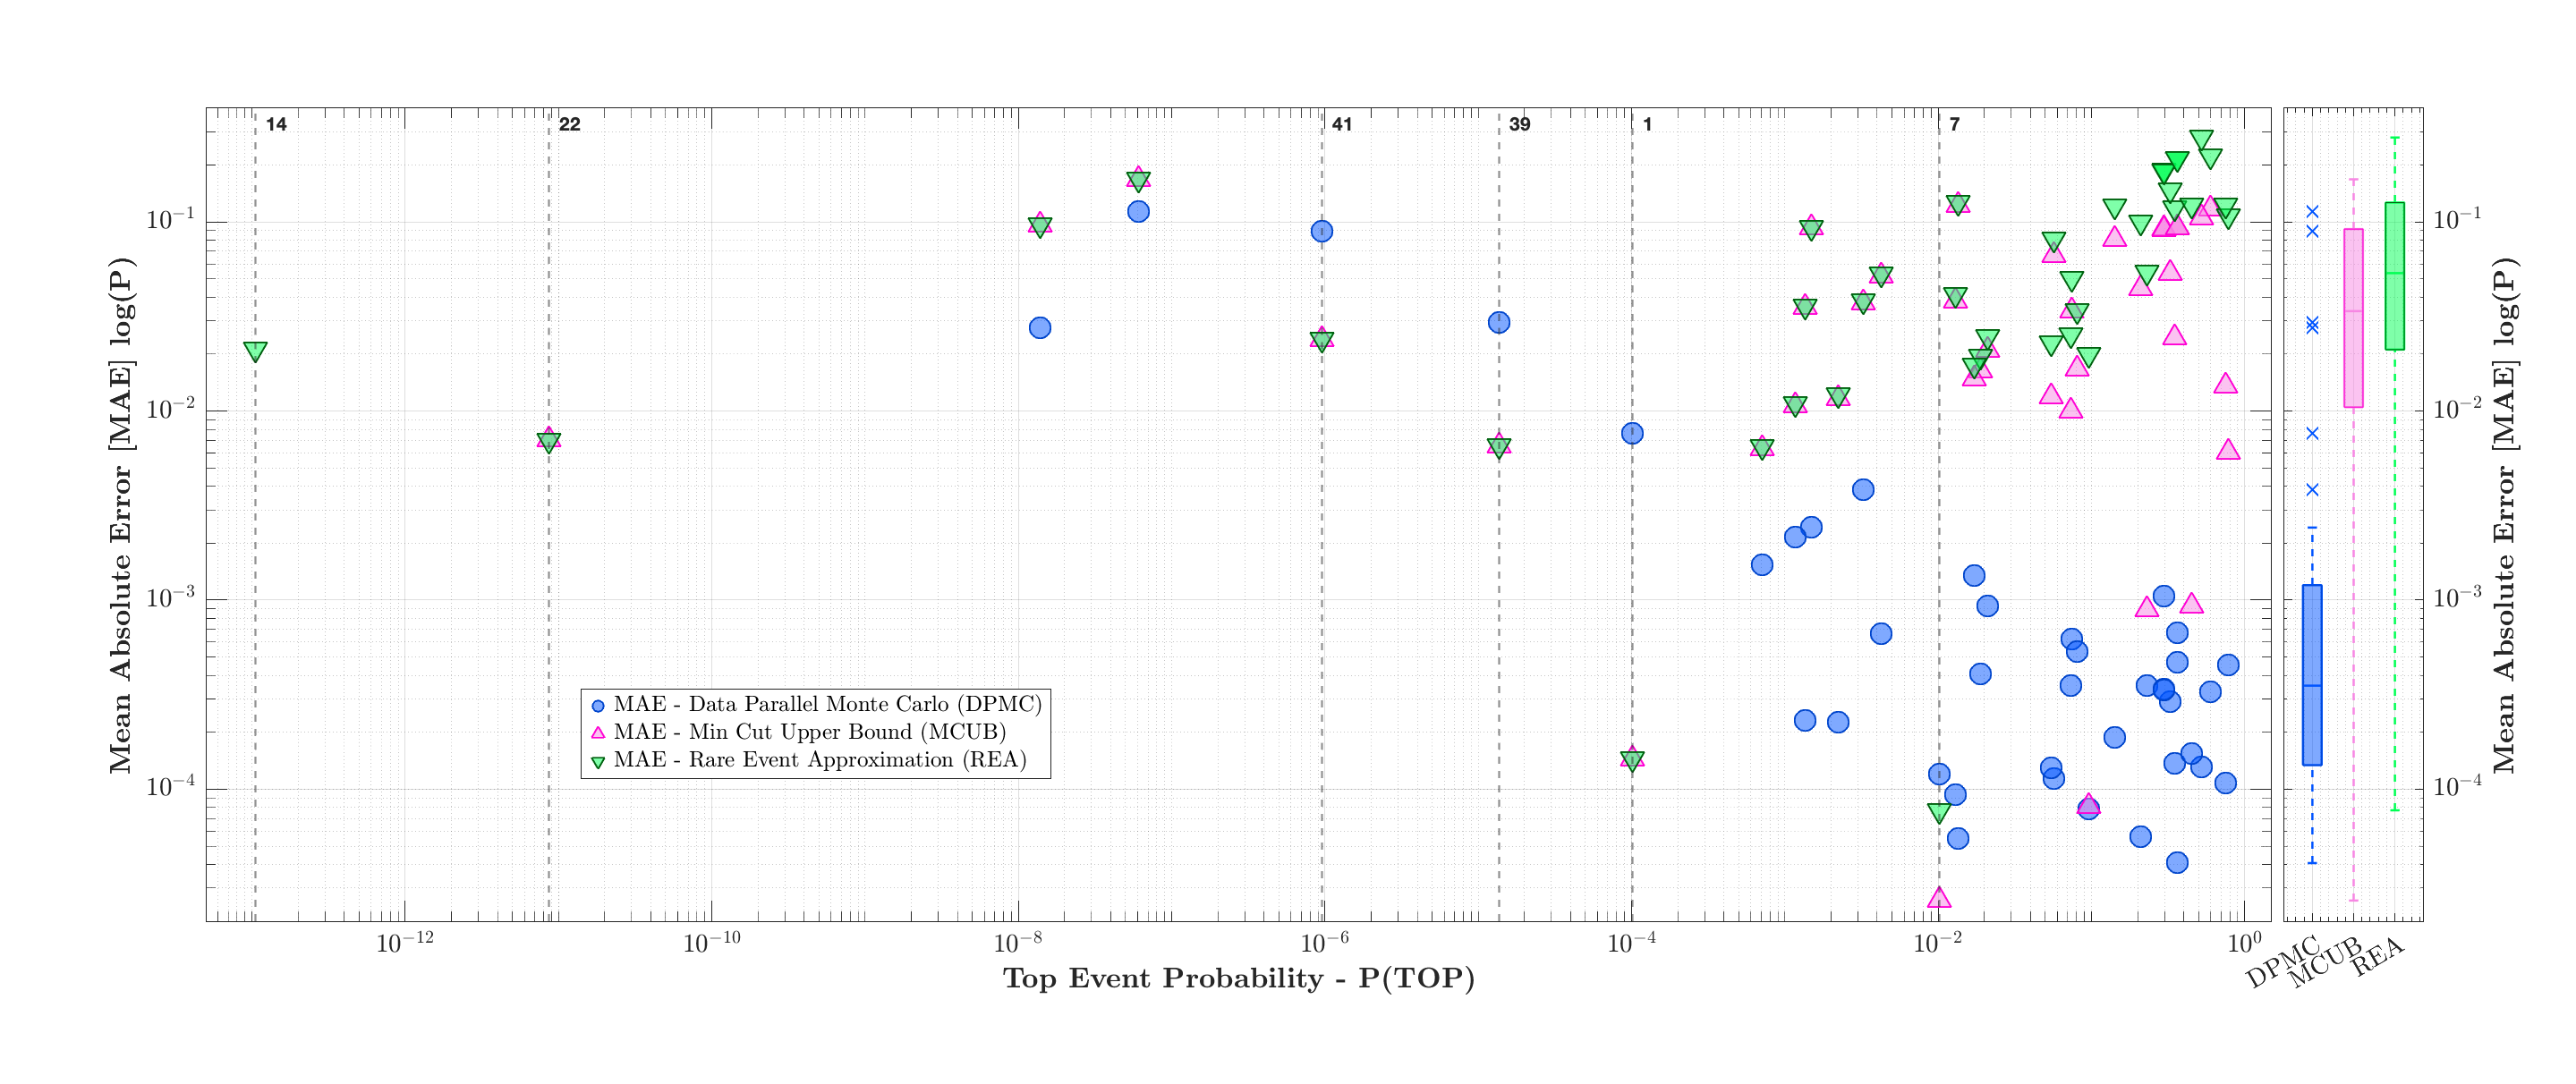
\includegraphics[width=1.2\textwidth]{parts/2_bruteforce/3_benchmark/error_vs_prob_detailed.png}
    \caption{Mean Absolute Error – Exact (BDD) vs Approximate Methods}
    \label{fig:mae_vs_logp}
\end{figure}
\end{landscape}

\input{parts/2_bruteforce/3_benchmark/4_mae}

% \part{Refinements}
\begin{sanskrit}
करत करत अभ्यास, जड़मति होत सुजान
\end{sanskrit}

\chapter{Variance Reduction}
\section{Dealing with Rare Events using Importance Sampling}
\subsection{Interplay between ultra-rare and ultra-frequent events - how they affect convergence}
\section{Sampling Correlated Events}
\chapter{Hardware Optimizations}

\input{parts/3_refinements/2_hw_opt/1_voter/_}

\part{Learning}

\chapter{Towards Parameter Learning}
\label{sec:parametric_learning_pra_model}

PRAs invariably involve uncertainty. When explicitly modeled, these uncertainties can be updated or inferred from evidence, engineering judgments, or reliability targets. We refer to such systematic updating of probability or frequency distributions across the PRA model as form of parametric learning.

Recall from (Section~\ref{sec:unified_pra_dag}) that we represent a PRA model as a PDAG. Let \(\boldsymbol{\theta}\) be the collection of parameters governing all relevant probabilities/frequencies in this PDAG. For an end-state \(S_j\), the model-based prediction under \(\boldsymbol{\theta}\) is
\[
P_{\mathcal{M}}\bigl(S_j \mid \boldsymbol{\theta}\bigr).
\]
If one also has observed or target frequencies \(\bigl\{p_{j}^{\mathrm{obs}}\bigr\}\), parametric learning seeks to reconcile this information with the model’s predictions by updating \(\boldsymbol{\theta}\). In a Bayesian setting, one may specify a prior distribution over \(\boldsymbol{\theta}\) and update this prior to a posterior distribution via the likelihood of observed end-state frequencies or other system-level evidence. Alternatively, one may adopt an optimization-based approach: define a loss or cost function that measures the discrepancy between \(\{p_{j}^{\mathrm{obs}}\}\) and \(\{P_{\mathcal{M}}(S_j \mid \boldsymbol{\theta})\}\), then minimize this loss with respect to \(\boldsymbol{\theta}\). Both perspectives aim to systematically adjust the PRA model’s probabilistic parameters so that end-state frequencies (or other risk metrics) remain consistent with available data or requirements. 

In the next section, we show how parametric learning over the PDAG can be setup as a constrained optimization problem.

\section{Parameter Learning as Constrained Optimization}
\label{sec:opt_formalization}

Each node \(X_i\) in the PDAG has an associated parameter \(\theta_i\), gathered into a vector  
\[
\boldsymbol{\theta}
\;=\;
(\theta_1,\;\theta_2,\;\dots,\;\theta_n).
\]
For a set of end-states \(\{S_j\}_{j=1}^m\), the model’s predicted probability under \(\boldsymbol{\theta}\) is  
\[
p_{j}^{\mathrm{pred}}\bigl(\boldsymbol{\theta}\bigr)
\;=\;
P_{\mathcal{M}}\bigl(S_j \mid \boldsymbol{\theta}\bigr).
\]
Suppose observed or target frequencies \(\bigl\{p_{j}^{\mathrm{obs}}\bigr\}\) are given. A discrepancy measure  
\[
d\!\bigl(p_{j}^{\mathrm{obs}},\,p_{j}^{\mathrm{pred}}(\boldsymbol{\theta})\bigr)
\]
compares the model’s predictions to these values. One can also add a regularization term \(\Psi(\boldsymbol{\theta})\) to encode additional constraints such as engineering limits or prior information. Let \(\Omega\) denote the feasible set for \(\boldsymbol{\theta}\), enforcing domain-specific requirements (e.g., probability normalization). Parameter learning then becomes the following constrained optimization problem:
\[
\min_{\boldsymbol{\theta} \,\in\, \Omega} 
\quad 
\sum_{j=1}^m
d\!\Bigl(
   p_{j}^{\mathrm{obs}},\,
   p_{j}^{\mathrm{pred}}(\boldsymbol{\theta})
\Bigr)
\;+\;
\Psi(\boldsymbol{\theta}).
\]
A solution \(\boldsymbol{\theta}^{*}\) in \(\Omega\) is sought that minimizes overall discrepancy while respecting any additional constraints. Gradient-based methods (when \(d\) is differentiable) or other solvers can be employed.

\input{parts/4_learning/1_param/1_demo}
\input{parts/4_learning/1_param/3_case_study}
\input{parts/4_learning/1_param/4_figs}

\section{Transformations}
\input{2_foundations/knowledge_compilation/transformation/as_nnf}
\input{2_foundations/knowledge_compilation/transformation/as_dnf_tree}
\input{2_foundations/knowledge_compilation/transformation/as_cnf}
\input{2_foundations/knowledge_compilation/transformation/as_dnnf}
% \subsection{\color{blue}{And-Inverter Graphs}}
\input{2_foundations/knowledge_compilation/transformation/as_dd/_}

%%---------------------------------------------------------------------------%%
%%  Bibliography 
%% or use BibTeX
\bibliography{references}
\bibliographystyle{apalike}

%%---------------------------------------------------------------------------%%
% Appendices
%\ensureoddstart
\restoregeometry

\appendix


\chapter{Revised Aralia Benchmark Plots}

In this chapter, we plot the the Monte--Carlo convergence experiments on the \emph{Aralia} fault--tree data set (Section~\ref{subsec:aralia_dataset}).  The revised study targeted a relative margin of error of $0.1\%$, that is, $\varepsilon = 10^{-3}\,\hat{p}$, at a $99\,\%$ confidence level with a wall--clock time limit of 60~s per model. The following figures collate the updated convergence traces for all 43 fault trees.

\begin{itemize}
  \item the sample mean estimate (solid colored line),
  \item the empirical $90\,\%$ and $99\,\%$ confidence bands (shaded regions)
  \item where available, the reference ``oracle/true'' probability (black dashed).
\end{itemize}


\begin{landscape}
\foreach \i in {1,...,9}{%%
  \begin{figure}[p]
      \centering
      \includegraphics[width=1\textwidth]{figs/convergence/e001p99/conv_fig_0\i.png}
      \caption{Aralia Fault Tree \i}
      \label{fig:conv_fig_\i}
  \end{figure}
}

\foreach \i in {10,...,43}{%%
  \begin{figure}[p]
      \centering
      \includegraphics[width=1\textwidth]{figs/convergence/e001p99/conv_fig_\i.png}
      \caption{Aralia Fault Tree \i}
      \label{fig:conv_fig_\i}
  \end{figure}
}
\end{landscape}

%\newgeometry{margin=1in,lmargin=1.25in,footskip=\chapterfootskip, includehead, includefoot}

% Can remove or add

\restoregeometry

%%---------------------------------------------------------------------------%%

%%---------------------------------------------------------------------------%%
\backmatter
\end{document}